\documentclass[11pt,a4paper]{article}
\usepackage[margin=1in]{geometry}
\usepackage[T1]{fontenc}
\usepackage{lmodern}
\usepackage{microtype}
\usepackage{graphicx}
\usepackage{amsmath,amssymb}
\usepackage{booktabs,tabularx}
\usepackage{hyperref}
\hypersetup{colorlinks=true,linkcolor=blue,citecolor=blue,urlcolor=blue}
\setlength{\parskip}{0.35em}
\setlength{\parindent}{0pt}

\title{Unsupervised Learning for Analyzing Market Regimes\\[0.4em]
\large Cluster-Based Partitioning for Entropy Pooling}
\author{Lajos Galambos}
\date{Preliminary research note --- 16 November 2026}

\begin{document}
\maketitle

\begin{abstract}
This note studies clustering as an alternative to threshold-based partitioning when constructing market-state views for Entropy Pooling (EP). Separate low, middle and high bands for many variables produce a large Cartesian set of potential joint states, whose observed subsets can be small. We instead learn a joint partition and use each cluster's feature means and variances to calibrate EP views within the Fully Flexible Resampling framework described by Vorobets. The primary worked example uses 17 daily features and a robust-scaled, two-cluster K-means calibration following a standard-input model search. It mainly distinguishes calmer and stressed equity-market conditions. An expanded 51-feature experiment and balanced feature-subset experiments are treated as separate extensions. This is a descriptive result, not evidence of a universal two-regime structure or improved forecasts. The empirical question is whether cluster-based calibration produces more stable and useful scenario distributions than threshold-based alternatives.
\end{abstract}

\section{Problem and proposed contribution}

Market-state definitions combine interpretability with a statistical estimation problem. Thresholds such as the 25th and 75th percentiles are transparent, but separate partitions become difficult to populate as the number of conditioning variables increases. If variable \(m\) has \(I_m\) states, the number of potential joint states is
\begin{equation}
J=\prod_{m=1}^{M} I_m.
\end{equation}
For 17 features with three bands each, this is \(3^{17}=129{,}140{,}163\) potential combinations, rather than \(17^3\). These combinations are candidate states, not additional dimensions or simulated observations. Many can be empty, and statistics calculated from small occupied subsets can be uncertain.

This does not imply that EP itself must use only the observations in a state. EP reweights the historical scenario set. The concern is the quality of the state-profile estimates supplied as views and the concentration of the resulting posterior probabilities.

We propose learning a joint partition of the observed feature vectors instead of specifying a Cartesian grid of individual thresholds. The resulting groups supply state-specific moment targets. Clustering offers a practical way to control granularity, but does not automatically find the smallest sufficient number of regimes or the number explaining most variance. Feature selection, scaling, the clustering method and the choice of cluster count remain modelling decisions.

The contribution is an application and calibration extension of Vorobets's framework \cite{vorobets2025}, using the EP method introduced by Meucci \cite{meucci2008}. We retain the relative-entropy objective and Fully Flexible Resampling (FFR) procedure; we change how the partition and its profile-based views are obtained.

\section{Literature review and positioning}
\label{sec:literature}

This expanded narrative review connects probability reweighting, market-state resampling, regime identification and clustering validation. It emphasizes the object being clustered, the role of the resulting labels, and the evidence required before a statistical partition can support investment analysis. Financial clustering and combinations of clustering with EP predate this project. The narrower proposal is to investigate cluster-derived joint moment profiles as a calibration alternative within an existing state-dependent resampling framework.

\subsection{Entropy Pooling and conditional Flexible Probabilities}

Meucci \cite{meucci2008} develops EP as a way to incorporate views into a reference market distribution by minimizing relative entropy subject to constraints. The framework accommodates general, non-normal market scenarios and views on functions of market variables. Its relevant feature here is that scenario locations can remain fixed while their probabilities change. Clustering can contribute to view construction without replacing the underlying EP optimization.

Estimating a prior and specifying a view are different operations. A cluster profile estimated from a historical subset is an empirical conditioning target. Its use does not make it a forward-looking economic forecast, and matching imposed moments does not independently validate the reweighted asset distribution. These are implications for the proposed empirical design.

Meucci \cite{meucci2013} develops time- and market-conditional Flexible Probabilities, including crisp conditioning, kernel-style conditioning, exponential time weighting and their combination through EP. He also discusses ensembles of probability vectors. This directly precedes using historical subsets to obtain state-conditioned distributions. Conditioning on market information, smoothing hard subsets through reweighting, and combining time and state information are therefore established ideas.

The proposed change concerns how subsets are identified and how their multivariate profiles enter the constraints. Percentile bands provide a transparent reference. Clusters instead use a chosen feature geometry to identify groups jointly. Whether this improves moment-estimation stability, posterior concentration or the resulting asset distributions remains an empirical question.

\subsection{Conditional probabilities and multi-period resampling}

Vorobets \cite{vorobets2025} supplies the immediate application framework. On printed page 33, threshold-defined ranges produce moment targets for EP, and the resulting probabilities drive FFR. The multiple-state-variable extension permits several conditioning variables and combines separately calibrated probability vectors. Our application therefore extends a framework that already incorporates multivariate information.

Kristensen and Vorobets \cite{kristensenvorobets2025} formalize Time- and State-Dependent Resampling and analyze FFR as an instance of that class. Historical rows are sampled using state-specific probabilities, and sampled observations update the state. They establish properties of the resampling construction, including stationarity results within the specified model. These results do not independently verify that a particular learned partition or feature set generates accurate future market distributions.

Dependent-data resampling offers another benchmark. Politis and Romano \cite{politisromano1994} introduce the stationary bootstrap, based on blocks of random, geometrically distributed length, for inference from weakly dependent stationary observations. A block-based benchmark retains local historical sequences, whereas our FFR implementation generates paths through state-conditioned row selection and state updates. This comparison could help separate the contribution of state information from that of handling time dependence more carefully than an independent bootstrap.

Two changes should be distinguished in the current application: learning a joint partition and imposing simultaneous feature views in each EP solve. Comparing only the complete implementation against a percentile baseline would confound them. A useful experiment should vary partition construction and multivariate probability calibration separately while holding the data, prior and horizon fixed.

\subsection{Econometric regimes and the meaning of a market state}

Hamilton \cite{hamilton1989} models discrete, unobserved changes in the growth rate of a nonstationary economic series and develops inference for the latent state. This provides a central econometric reference for recurrent regimes. State inference is part of a probabilistic dynamic model; a state is not simply the nearest centre in a feature space.

Ang and Timmermann \cite{angtimmermann2012} review financial regime changes, emphasizing abrupt shifts, persistence and differences in return moments and dependence across regimes. Their discussion motivates evaluating state-conditioned distributions rather than assuming one stable set of unconditional parameters. It does not imply that every geometrically separated group corresponds to a distinct economic mechanism.

For our application, statistical states are operational labels with profiles and associated probabilities. Economic descriptions can be examined after estimation, but their absence does not prevent labels from indexing resampling. Conversely, an intuitive stress label is not evidence of predictive value. Economic coherence, persistence and downstream risk relevance require evaluation beyond the partition-selection criterion.

Contemporaneous assignment and forecasting must also be distinguished. K-means assigns an observed feature vector using fitted centres. A regime-switching model specifies dynamics for latent states, while FFR supplies model-implied transitions through its probability library. Similar historical state plots therefore need not imply equivalent forecasting models.

\subsection{Financial clustering: dates, dependence structures and assets}

M\"unnix et al.\ \cite{munnix2012} identify market states by clustering correlation structures measured over time windows. Their study of S\&P 500 stocks demonstrates that recurring patterns of market dependence can be described as statistical states. The clustered objects are window-specific correlation matrices. Our application instead clusters dated vectors of macro-financial and technical features, then calculates conditioning moments within the groups. These approaches encode different definitions of similarity and market state.

Asset clustering is a distinct strand. L\'opez de Prado \cite{lopezdeprado2016} introduces Hierarchical Risk Parity, using the structure in asset covariance information to construct diversified portfolios. Its learned groups organize assets rather than historical dates. Asset-allocation methods using clusters should therefore be distinguished from learning time-indexed state partitions.

A particularly relevant antecedent is Mba and Angaman \cite{mbaangaman2023}, who combine K-means classification and EP in a cryptocurrency portfolio study. They cluster cryptocurrency assets to construct portfolios and formulate EP volatility views using GARCH forecasts. This establishes prior use of the methods together. Our narrower distinction is to cluster historical dates, derive EP moment targets from their multivariate profiles, and use the resulting weights in FFR. That distinction supports a research question rather than a broad first-use claim.

The unit of analysis is therefore essential: groups of assets, correlation windows and dated feature vectors solve different problems. Literature comparisons should identify both the clustered objects and the way their grouping enters subsequent investment analysis.

\subsection{Temporal clustering and persistent states}

Static K-means groups observations by their feature values without penalizing switches between labels on consecutive dates. A compact partition can consequently produce an unstable state sequence. Whether this is problematic depends on the application: rapidly changing labels can describe shocks, but may be less useful as persistent regime signals.

Nystrup, Kolm and Lindstr\"om \cite{nystrup2021} develop feature selection in jump models, jointly estimating feature relevance, parameters and the state sequence while incorporating sequential ordering. Their work addresses both potentially noisy features and persistence. It provides a benchmark that changes state estimation itself rather than merely adjusting probabilities after static clustering.

Ayd{\i}nhan et al.\ \cite{aydinhan2024} extend statistical jump models from discrete state assignments to probability vectors over regimes. This offers a soft-state alternative for downstream applications. Such models are candidates for comparison here rather than components of the current K-means implementation.

Membership probabilities and scenario probabilities are different objects. A soft-state model describes uncertainty about the state of an observation. EP assigns weights to historical scenarios under a profile. The latter is not automatically a calibrated estimate of the former; combining them requires an explicit rule and validation.

\subsection{PCA, feature geometry and the K-means objective}

Lloyd's least-squares quantization work \cite{lloyd1982} supplies an algorithmic foundation for alternating partition and representative-point estimation. The relevant connection is the squared-distance objective. It gives a reproducible geometric definition of similarity, rather than an economic theory of regimes. Scaling and feature composition therefore help define what the method regards as a meaningful difference.

Ding and He \cite{dinghe2004} establish a connection between PCA and continuous relaxations of K-means indicators and derive bounds for the clustering objective. This supports treating dimension reduction and clustering as related operations. It does not establish that a particular explained-variance cutoff recovers the best economic regimes or the cluster count.

Chang \cite{chang1983} shows, in a mixture setting, that PCs with larger eigenvalues need not contain the most information for distinguishing groups. This motivates a limitation of the cutoff rule: high total variance and useful state separation can lie in different directions.

Three decisions should thus be recorded separately: the features and transformations defining the geometry, the retained PCA dimension, and the preferred clustering under a declared score. A variance cutoff is a transparent rule, but should be tested alongside alternatives. Skewness, tails and related feature families affect covariance and squared distances. Several volatility descriptors, for example, can emphasize market stress even when the research question concerns broader macroeconomic regimes.

\subsection{Selection, stability and distributional evaluation}

Rousseeuw \cite{rousseeuw1987} introduces silhouettes to assess within-cluster cohesion and between-cluster separation, with average width providing a possible selection criterion. This underlies the current K-means count search. A good score establishes a preference under a geometry, rather than a uniquely true number of states.

Tibshirani, Walther and Hastie \cite{tibshirani2001} propose the gap statistic, comparing within-cluster dispersion with a reference null distribution. This supplies an alternative count-selection rule and highlights the role of the benchmark. Disagreement between rules would be informative about the resolution supported by the data.

Von Luxburg \cite{luxburg2010} reviews clustering stability and the theoretical subtleties of using it for model selection. Reproducibility across initializations, sensitivity to changes in the sample, and stability across rolling windows answer different questions. Repeating a fixed historical sample under several seeds addresses only the first; it cannot establish stable state definitions across market histories.

Distributional evaluation should assess the complete pipeline. Gneiting and Raftery \cite{gneitingraftery2007} develop proper scoring rules for probabilistic forecasts. This motivates using an appropriate distributional score, such as the continuous ranked probability score, to evaluate conditional empirical return distributions. Rolling or expanding training windows should preserve the temporal order of estimation and evaluation.

Rockafellar and Uryasev \cite{rockafellaruryasev2000} provide a scenario-compatible CVaR optimization approach. Here, CVaR is initially a risk summary of resampled asset distributions, not a demonstrated portfolio-allocation improvement. A larger difference between the states' CVaR values alone does not establish better forecast calibration.

Together, these works suggest evaluation at three levels: partition quality, profile and probability stability, and out-of-sample asset-distribution performance. The criteria can disagree. Useful improvements should survive through the final stage while retaining economic and operational relevance.

\subsection{Positioning and the remaining research question}

Table~\ref{tab:literature-position} summarizes selected relationships to this project. It is a positioning comparison rather than an exhaustive classification.

\begin{table}[htbp]
\centering
\small
\begin{tabularx}{\textwidth}{@{}p{0.26\textwidth}XX@{}}
\toprule
Literature & Object or mechanism & Distinction here\\
\midrule
EP and Flexible Probabilities \cite{meucci2008,meucci2013}
& Historical weights and conditional views
& Cluster profiles supply targets.\\[3pt]
FFR \cite{vorobets2025,kristensenvorobets2025}
& State-dependent row resampling
& Retain the framework; change calibration.\\[3pt]
Regime switching \cite{hamilton1989,angtimmermann2012}
& Dynamic latent states
& Geometric assignment is a different estimator.\\[3pt]
Correlation-state clustering \cite{munnix2012}
& Window-specific dependence matrices
& Cluster daily feature vectors.\\[3pt]
Clustering with EP \cite{mbaangaman2023}
& Asset groups for portfolio construction
& Cluster dates to calibrate state profiles.\\[3pt]
Jump models \cite{nystrup2021,aydinhan2024}
& Temporally ordered or soft states
& Benchmark for static K-means.\\
\bottomrule
\end{tabularx}
\caption{Selected literature and its relationship to the proposed application.}
\label{tab:literature-position}
\end{table}

The contribution is best framed as an empirical calibration study within the established EP/FFR architecture. It examines whether learned joint groups produce more useful moment targets and state-conditioned distributions than specified threshold partitions. Existing financial clustering and clustering--EP applications preclude a broad first-use claim. A wider search would be required before asserting priority even for the narrower construction.

The main hypothesis requires a controlled comparison. Replacing percentile groups with clusters, replacing probability mixing with simultaneous EP views, truncating PCA, changing scaling and selecting a different number of states can each alter results. Changing all of these together evaluates a complete configuration, but does not isolate the effect of clustering.

The method also does not eliminate judgement. It relocates some decisions from individual thresholds to feature construction, representation, count selection and validation. Its potential value is a reproducible calibration of a manageable set of joint scenarios, supported by transparent diagnostics and forward evaluation. Economic narratives can aid interpretation; usefulness ultimately depends on the distributions and decisions the framework is intended to support.


\section{Mathematical formulation}

\subsection{Preprocessing and PCA dimension choice}

Index the aligned observations by $t=1,\ldots,T$. Let $y_t\in\mathbb R^p$ contain the clustering features, $r_t$ the output asset's daily log return, and $x_t\in\mathbb R^d$ the EP conditioning features excluding that return. Construct features from raw observations, align complete dates, scale the clustering inputs, and apply mean-centred PCA. In the current implementation, the S\&P 500 close becomes a daily log return; other inputs retain their level, ratio or precomputed descriptor definitions. A common log-return transformation is not imposed on all features. The feature construction, standard and robust scaler formulas, and PCA transformation are detailed in Appendix~\ref{app:preprocessing}.

For ordered eigenvalues $\lambda_1\geq\cdots\geq\lambda_p\geq0$ of the scaled-feature covariance, a declared cumulative explained-variance cutoff $\eta$ selects the smallest retained dimension:
\begin{equation}
\widehat L(\eta)=\min\left\{L\in\{1,\ldots,p\}:
\frac{\sum_{\ell=1}^{L}\lambda_\ell}{\sum_{\ell=1}^{p}\lambda_\ell}\geq\eta\right\}.
\label{eq:pca-dimension}
\end{equation}
K-means receives the retained scores $u_t\in\mathbb R^{\widehat L}$, without whitening. For example, a 70\% cutoff selects four PCs in the original 17-feature data: the first four explain 70.77\% after standard scaling and 75.37\% after robust scaling.

This is a variance-retention rule, rather than evidence that the dimension is best for separating regimes or for economic interpretation. The scaling, cutoff and validation geometry must be stated explicitly. Fix the PCA dimension $\widehat L$ before selecting the separate cluster count $\widehat K$; EP profiles are subsequently calculated from the conditioning features $x_t$.

\subsection{Cluster-based partition and state profiles}

For K-means, the fitting criterion is
\begin{equation}
\min_{\{a_k\},\,\{c_t\}}
\sum_{t=1}^{T}\|u_t-a_{c_t}\|_2^2,
\qquad c_t\in\{0,\ldots,K-1\}.
\end{equation}
The cluster count is selected from candidate fits, rather than fixed at two. For the retained PCA dimension $\widehat L$, let $\widehat{\mathcal P}_{K,\widehat L}$ be the fitted partition for candidate $K\in\mathcal K$ and let $\mathcal S$ be a declared selection score. For a score where larger values are preferred, select
\begin{equation}
\widehat K=\underset{K\in\mathcal K}{\arg\max}\,
\mathcal S(\widehat{\mathcal P}_{K,\widehat L}).
\label{eq:select-k}
\end{equation}
For example, silhouette can select among a finite set of candidate counts. K-means requires a specified candidate $K$ for each fit; the selection step makes the final count data-dependent within the chosen search set and criterion. The selected partition is statistically preferred under the specified geometric validation criterion among the candidate configurations examined. This criterion-based preference need not coincide with the most economically interpretable or decision-relevant regime classification. A well-separated partition may emphasize market stress while overlooking economically meaningful distinctions in inflation, growth or monetary policy. Economic interpretation and usefulness for scenario analysis therefore require separate evaluation; the selection does not establish a universally optimal partition or a uniquely true number of economic regimes.

Given the selected fit, assign
\begin{equation}
c_t=\underset{k\in\{0,\ldots,\widehat K-1\}}{\arg\min}\,
\|u_t-a_k\|_2^2,
\qquad
\mathcal C_k=\{t:c_t=k\},\qquad N_k=|\mathcal C_k|.
\end{equation}
Ties are resolved deterministically. Cluster labels identify groups and carry no numerical ordering of risk. Equations below apply to every $k=0,\ldots,\widehat K-1$, yielding $\widehat K$ profile-specific EP probability vectors. Two clusters appear only as the current empirical example.

For each cluster, calculate the conditioning-feature mean and population variance vectors:
\begin{equation}
\boldsymbol\mu_k=\frac{1}{N_k}\sum_{t\in\mathcal C_k}x_t,
\qquad
\boldsymbol v_k=\frac{1}{N_k}\sum_{t\in\mathcal C_k}
(x_t-\boldsymbol\mu_k)\odot(x_t-\boldsymbol\mu_k).
\label{eq:profiles}
\end{equation}
Here \(\odot\) denotes elementwise multiplication. All components of a profile are estimated from the same joint group of observations. These are empirical scenario targets, rather than externally supplied forecasts. The labels are learned in PCA space, while the EP moments are calculated from the corresponding conditioning-feature observations $x_t$; an inverse PCA reconstruction is not required.

The complete sequence can be summarized as
\begin{equation}
\begin{aligned}
\{w_\tau\}
&\xrightarrow{g,\,\mathcal I}Y
\xrightarrow{\mathrm{scale}}S
\xrightarrow{\mathrm{PCA},\,\eta}U_{\widehat L},\\
U_{\widehat L}
&\xrightarrow{\mathrm{select}\ K}
(\widehat K,\{\mathcal C_k\})
\xrightarrow{\mathrm{profile}\ X}
\{(\boldsymbol\mu_k,\boldsymbol v_k)\}
\xrightarrow{\mathrm{EP}}\{q^{(k)}\}.
\end{aligned}
\label{eq:complete-pipeline}
\end{equation}
Here $S$ and $U_{\widehat L}$ have the scaled observations and retained PCA scores as rows. The PCA dimension is selected first under the variance-retention rule; candidate K-means fits then receive that fixed PCA representation.

\subsection{Entropy Pooling with cluster-derived views}

Use a positive prior \(p_t\), for example uniform probabilities or exponential decay:
\begin{equation}
p_t=
\frac{\exp[-(\log 2)(T-t)/\tau]}
{\sum_{s=1}^{T}\exp[-(\log 2)(T-s)/\tau]}.
\label{eq:prior}
\end{equation}
The current example sets \(\tau=T/2\). For each cluster \(k\), solve
\begin{equation}
\begin{aligned}
q^{(k)}=\underset{q\in\mathbb R^T}{\arg\min}\quad&
D_{\mathrm{KL}}(q\|p)
=\sum_{t=1}^{T}q_t\log\frac{q_t}{p_t}\\
\text{subject to}\quad&
q_t\geq0,\qquad \sum_{t=1}^{T}q_t=1,\\
&\sum_{t=1}^{T}q_t x_t=\boldsymbol\mu_k,\\
&\sum_{t=1}^{T}q_t(x_t\odot x_t)
\leq\boldsymbol\mu_k\odot\boldsymbol\mu_k+\boldsymbol v_k.
\end{aligned}
\label{eq:ep}
\end{equation}
The inequality is componentwise. Given the mean equalities, it imposes upper bounds on the individual feature variances, following the chapter's specification. Exact variance matching would instead require second-moment equalities.

For \(X\in\mathbb R^{T\times d}\) with rows \(x_t^\top\), the matrices passed to the existing EP solver are
\begin{equation}
A=\begin{bmatrix}\mathbf1^\top\\X^\top\end{bmatrix},
\quad b_k=\begin{bmatrix}1\\\boldsymbol\mu_k\end{bmatrix},
\quad G=(X\odot X)^\top,
\quad h_k=\boldsymbol\mu_k\odot\boldsymbol\mu_k+\boldsymbol v_k,
\end{equation}
so the constraints are \(Aq=b_k\) and \(Gq\leq h_k\). Each solve uses the full historical scenario set. It need not assign zero probability outside \(\mathcal C_k\).

These views do not fix all covariances or the full joint distribution. Historical feature--return pairings remain intact when rows are reweighted, while their weighted dependence can change. The entropy-based effective number of scenarios,
\begin{equation}
\operatorname{ENS}(q)=\exp\!\left(-\sum_{t=1}^{T}q_t\log q_t\right),
\end{equation}
is a concentration diagnostic, not the objective used in \eqref{eq:ep}. It also differs from the inverse-concentration measure \(1/\sum_t q_t^2\), which the notebook currently reports.

\subsection{Comparison with threshold-based state construction}

On printed page 33 of Vorobets \cite{vorobets2025}, a scalar state variable \(z_t\) is partitioned using thresholds \(v_1<v_2\). With the example's percentile thresholds, the observation sets are
\begin{equation}
\begin{aligned}
\mathcal C_L&=\{t:z_t\leq v_1\},\\
\mathcal C_M&=\{t:v_1<z_t\leq v_2\},\\
\mathcal C_H&=\{t:z_t>v_2\},
\qquad v_1=Q_{0.25}(z),\quad v_2=Q_{0.75}(z).
\end{aligned}
\label{eq:threshold}
\end{equation}
Each set supplies a mean and a population variance for the state variable, which become EP views. The proposed extension replaces the sets in \eqref{eq:threshold} with a learned multivariate partition.

The intended partitioning comparison is
\[
\begin{array}{c}
\text{Threshold partition}\ \longrightarrow\ \text{State profiles}\
\longrightarrow\ \text{EP}\ \longrightarrow\ \text{FFR}\\[4pt]
\text{Cluster partition}\ \longrightarrow\ \text{State profiles}\
\longrightarrow\ \text{EP}\ \longrightarrow\ \text{FFR}.
\end{array}
\]
Vorobets already supports multiple state variables in Section 3.2.1.1. That construction combines separately calibrated per-variable EP probability vectors through a weighted linear mixture. Our current implementation instead imposes all conditioning-feature views simultaneously in one solve per cluster. A controlled empirical comparison must therefore distinguish the effect of changing the partition from the effect of changing the multivariate calibration procedure.

\subsection{Asset distributions and multi-period resampling}

The one-day simple-return distribution associated with profile \(k\) is
\begin{equation}
\widehat F_k(a)=
\sum_{t=1}^{T}q_t^{(k)}
\mathbf1\{\exp(r_t)-1\leq a\}.
\end{equation}
For an \(H\)-step FFR path starting in state \(s_0\), sample a row index and update the state:
\begin{equation}
I_h\sim\operatorname{Categorical}(q^{(s_{h-1})}),
\qquad s_h=c_{I_h},
\qquad
R_H=\exp\!\left(\sum_{h=1}^{H}r_{I_h}\right)-1.
\end{equation}
The implicit transition probabilities are
\begin{equation}
P_{k\ell}=\sum_{t:c_t=\ell}q_t^{(k)}.
\end{equation}
They follow from EP weights and sampled-row labels, rather than counts of consecutive historical state changes. Multi-period distributions condition on the initial state and allow later state changes. Risk summaries include simple-return moments and 90\% and 95\% CVaR, measured as tail losses without demeaning.

\section{Study design and model comparison}
\label{sec:study-design}

\subsection{Primary example and separate extensions}

The primary worked example is the original 17-feature experiment in \texttt{02\_clustering\_analysis.ipynb}, with 3,738 complete observations from 6 October 2011 to 2 October 2026. Its selected robust K-means calibration already supplies the profiles used in the EP/FFR demonstration. Keeping this example as the main application maintains a traceable sequence from model comparison to profiles and scenario probabilities. It is not chosen because its scores can be compared favourably with a different feature universe.

The expanded study in \texttt{03\_random\_feature\_clustering.ipynb} has a different role. Its full-panel fit uses 50 candidate features plus the S\&P 500 log return on 3,630 common dates. Its randomized fits use five macro/market features, five technical features and the same mandatory return, giving eleven inputs per draw. Seven positive risk descriptors are logged in this extension before scaling; the original study does not apply those additional logs. These experiments change both the feature definitions and the complete-case sample. Their native silhouettes therefore cannot be ranked against the original experiment as if they were one model-selection contest.

\begin{table}[htbp]
\centering
\small
\begin{tabularx}{\textwidth}{@{}p{0.22\textwidth}XX@{}}
\toprule
Experiment & Configuration & Role in the paper\\
\midrule
Original, notebook 02 & 17 features; robust K-means calibration; all 16 informative PCs; selected $K=2$ & Primary detailed profiles and implemented EP/FFR example.\\[3pt]
Full panel, notebook 03 & 51 inputs; standard scaling; all informative PCs; own count/model search & Expanded benchmark; its calibrations are sensitivity checks.\\[3pt]
Feature draws, notebook 03 & $5+5$ randomly drawn features plus the fixed return; standard scaling; own count search & Sensitivity to feature choice, memberships and profiles.\\[3pt]
Return only, notebook 03 & Standardized S\&P 500 log return; own model search & Control for separation attributable to returns alone.\\
\bottomrule
\end{tabularx}
\caption{Reporting roles. Each experiment keeps its own feature map, sample, selection rule and labels. The original worked example is not a fitted model that is reused unchanged in the expanded experiments.}
\label{tab:experiment-roles}
\end{table}

\subsection{Original model search and a transparent population screen}

Five model families were evaluated, with three-cluster starting fits for the fixed-count methods and an initial DBSCAN configuration. The standard-input search contains 85 candidates, summarized in Table~\ref{tab:original-grid}. StandardScaler is fitted to all 17 inputs. Models receive all 16 informative, unwhitened PCA scores, so this rotation preserves Euclidean distances rather than truncating at four PCs. The VIX term-spread identity accounts for the redundant direction. Scores are calculated on the original 17 standardized features, excluding DBSCAN noise and reporting its coverage. AIC/BIC are compared only within the same GMM representation.

\begin{table}[htbp]
\centering
\small
\begin{tabularx}{\textwidth}{@{}lXrl@{}}
\toprule
Model & Standard-input grid & Fits & Selection\\
\midrule
K-means & $K=2,\ldots,8$; 20 starts; seed 1 & 7 & Highest silhouette\\[3pt]
K-medoids & $K=2,\ldots,8$; FasterPAM; seeds 1, 7 & 14 & Highest silhouette\\[3pt]
Hierarchical & $K=2,\ldots,8$; Ward, average, complete & 21 & Highest silhouette\\[3pt]
GMM & $K=2,\ldots,8$; full, tied, diagonal, spherical covariance & 28 & Lowest eligible BIC\\[3pt]
DBSCAN & Minimum samples 5, 10, 20; neighbour-distance quantiles 0.50, 0.65, 0.80, 0.90, 0.95 & 15 & Highest eligible silhouette\\
\bottomrule
\end{tabularx}
\caption{The original search, not an exhaustive inventory of clustering methods or parameter settings. GMM uses three starts, at most 500 iterations, covariance regularization $10^{-5}$ and seed 1.}
\label{tab:original-grid}
\end{table}

The original notebook's eligibility flag imposed population/coverage restrictions on DBSCAN but did not impose a common minimum population on every method. Consequently, its largest raw silhouette is 0.739 for complete-linkage hierarchical clustering, with just nine observations in the smaller group. That result remains visible in the complete inventory; it is not the preferred calibration for the present profile-estimation exercise.

For this paper's reporting comparison, apply the same population screen to every saved candidate: at least two clusters, finite silhouette, at least 80\% assigned coverage and at least $\max(20,\lceil0.01T\rceil)=38$ observations in every cluster; GMM must also converge. This is an explicitly retrospective reporting choice, not a rule that was prespecified in notebook 02. The threshold is a practical guard against extremely thin profiles, not a guarantee of reliable tail estimation. Its sensitivity remains to be examined. Reconsider all saved candidates under this screen, rather than discarding a model family merely because its original winner fails. The resulting hierarchical selection is Ward with $K=2$; no DBSCAN candidate passes. No model is refitted to produce this reporting comparison.

\begin{table}[htbp]
\centering
\small
\begin{tabularx}{\textwidth}{@{}Xrrrrrr@{}}
\toprule
Model & $K$ & Sil. & CH & DB & Min. $N_k$ & Cover. (\%)\\
\midrule
K-means & 2 & 0.329 & 1151.3 & 1.493 & 739 & 100.0\\
K-medoids & 8 & 0.171 & 550.8 & 1.753 & 213 & 100.0\\
Hierarchical (Ward) & 2 & 0.293 & 1014.4 & 1.665 & 863 & 100.0\\
GMM & 8 & 0.153 & 578.8 & 1.727 & 39 & 100.0\\
DBSCAN & --- & --- & --- & --- & --- & ---\\
\midrule
\textbf{K-means, robust}$^{*}$ & 2 & 0.342 & 1145.1 & 1.455 & 671 & 100.0\\
\bottomrule
\end{tabularx}
\caption{Original 17-feature experiment: per-model selections from the saved standard-input tuning grid after the retrospective population screen. Silhouette and Calinski--Harabasz (CH) are higher-is-preferred; Davies--Bouldin (DB) is lower-is-preferred. All scores use the same original 17 standardized features and all assigned dates. No DBSCAN candidate meets the paper screen. $^{*}$The robust K-means row is the detailed worked example: a fixed-$K$ calibration of the standard winner, not a renewed count search.}
\label{tab:original-selected-models}
\end{table}


\subsection{Configuration demonstrated in detail}

Use standard-scaled K-means with selected $K=2$ as the searched reference, and its robust-scaled $K=2$ calibration as the primary worked EP example. The reference has the highest silhouette among the screened standard-input per-family selections. The robust calibration improves silhouette from 0.329 to 0.342 and Davies--Bouldin from 1.493 to 1.455 in the same evaluation geometry; Calinski--Harabasz decreases slightly. The choice is thus supported by the declared geometric and population diagnostics, rather than dominance on every metric or investment usefulness.

The detailed calibration fits median/IQR RobustScaler to the same 17 feature columns, retains all 16 informative PCs without whitening, and fits K-means with $K=2$, 20 starts and seed 1. The count is inherited from the standard search; it is not reselected under robust scaling. Its ARI with the standard reference is 0.916. The original standard configuration is unchanged across the three tested initialization seeds (pairwise ARI 1); this seed check does not establish seed stability of the robust calibration. PCA95 is a further fixed-settings check, retaining ten standard PCs and leaving the K-means assignments nearly unchanged (ARI 0.996 with the standard reference).

In this note, ``preferred configuration'' means the selected, adequately populated worked example among the examined configurations. It does not mean the global optimum across models, the statistically proven number of economic regimes, or the most useful EP calibration. The full 20-row starting/tuned/calibration inventory and its saved numerical sources appear in Appendix~\ref{app:model-inventory}. Expanded-panel robustness, financial-profile tests and a controlled threshold-versus-cluster EP comparison remain separate layers of evidence; none is substituted for the others.

\section{Detailed worked example and interpretation}
\label{sec:preliminary}

The primary example follows the configuration fixed in Section~\ref{sec:study-design}: 17 features, 3,738 complete daily observations, robust scaling, all 16 informative PCs and the $K=2$ calibration inherited from the standard-input search. It does not use the illustrative four-PC/70\% cutoff. Cluster memberships are learned in that robust PCA geometry; profiles are calculated from the corresponding original feature observations, and geometric scores use the common 17-feature standard-scaled geometry.

The calibration has silhouette $0.342$ and Davies--Bouldin $1.455$, with all observations assigned. Its cluster sizes are:
\begin{center}
\begin{tabular}{lrr}
\toprule
Cluster & Observations & Share (\%)\\
\midrule
0 & 3,067 & 82.05\\
1 & 671 & 17.95\\
\bottomrule
\end{tabular}
\end{center}
Figure~\ref{fig:cluster-timeline} shows when each cluster appears in the historical sample.
\begin{figure}[htbp]
\centering
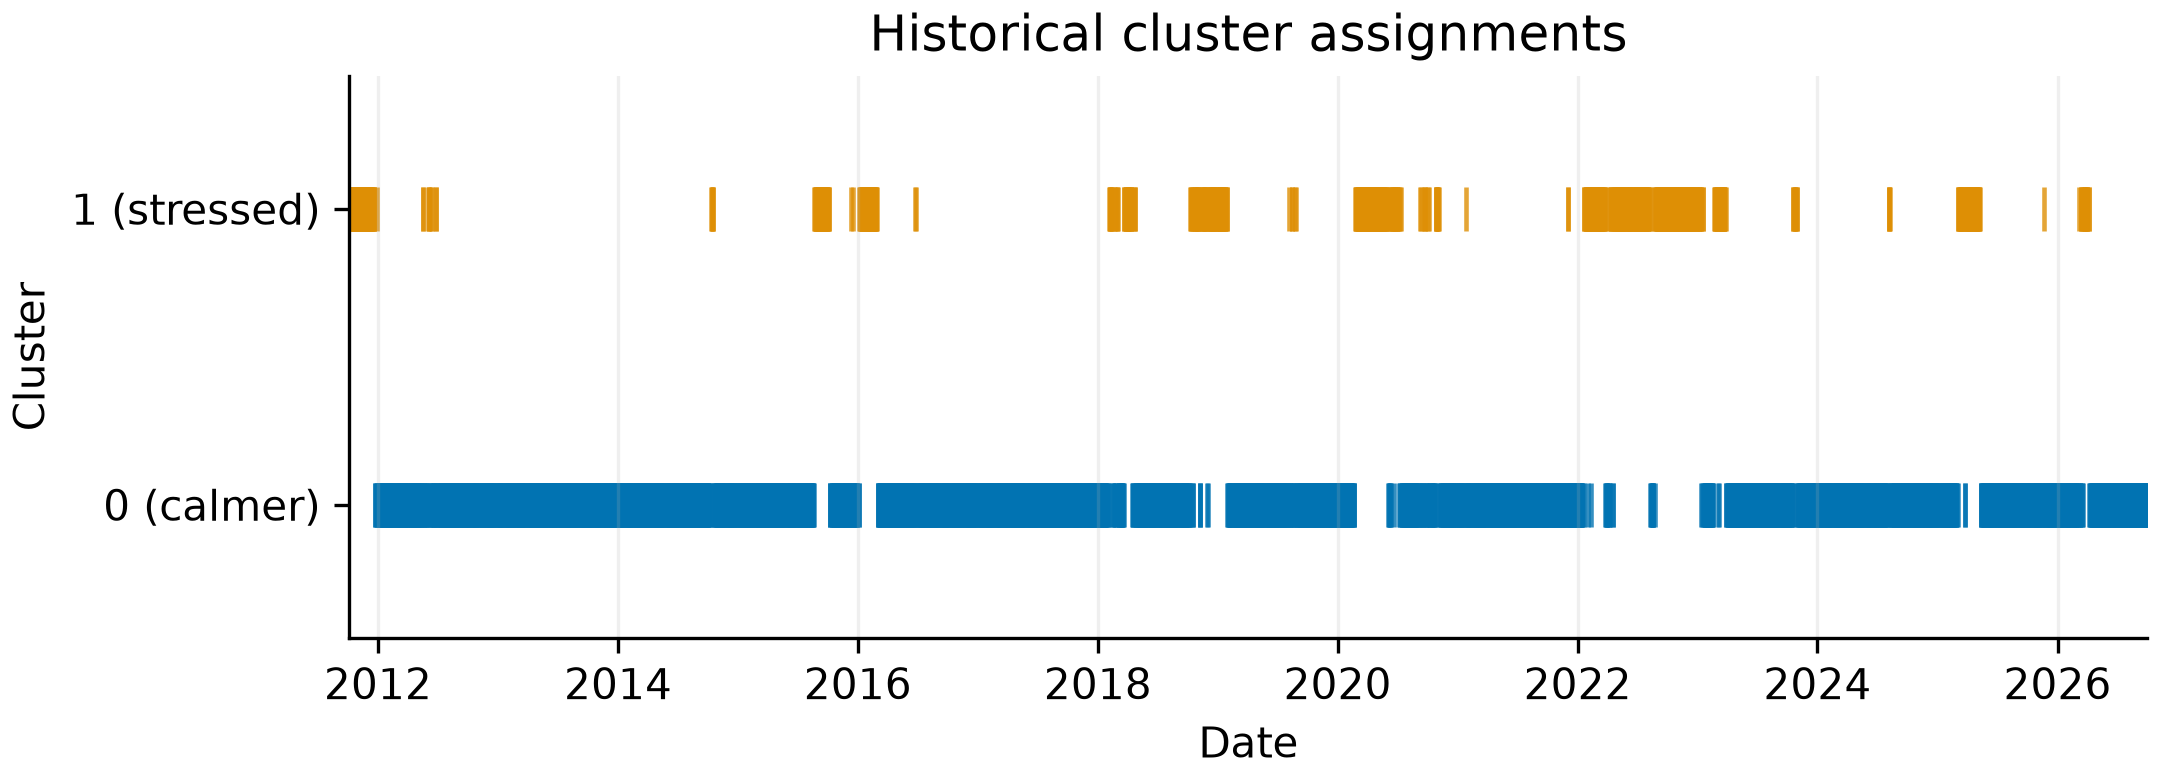
\includegraphics[width=\textwidth]{images/cluster_timeline.png}
\caption{Daily assignments from robust K-means with $K=2$, from 6 October 2011 to 2 October 2026. Each mark represents an observed date assigned to cluster 0 (calmer, 3,067 observations) or cluster 1 (stressed, 671 observations). Only complete feature dates are shown; missing dates are not filled. The labels are fitted on the full sample and are descriptive.}
\label{fig:cluster-timeline}
\end{figure}

The larger cluster is relatively calm. The smaller cluster has higher volatility, deeper drawdowns and negative average momentum. Their inflation and real-yield profiles are less distinct. This suggests a coarse market-stress partition, rather than a complete classification of macroeconomic regimes.

The two-cluster choice is provisional within the configurations examined. It does not establish that two clusters explain most variance, are the minimum number of regimes, or suffice for every asset and risk-management question. PCA variance retention and cluster-count selection answer different questions.

\paragraph{Modest silhouette and possible underfitting.}
The selected configuration's average silhouette of $0.342$ is modest, rather than evidence of sharply separated states. Silhouette compares within-cluster distances with distances to the nearest alternative cluster \cite{rousseeuw1987}; the positive average indicates some separation, but being preferred among the tested configurations does not imply strong absolute cluster quality. The average alone also does not reveal how many individual observations have near-zero or negative silhouettes. Per-cluster silhouette distributions are therefore needed to assess ambiguous assignments.

This limited separation raises a concern about whether K-means captures enough of the relevant structure. Underfitting is one possibility: the two groups may pool distinct subgroups whose differences matter for EP moment views. However, a modest silhouette does not diagnose underfitting or establish that increasing $K$ will improve the model. It can also reflect overlapping or continuous market conditions, the chosen feature geometry, or a mismatch between the data structure and the K-means distance-based partition. The large cluster containing 82.05\% of observations warrants further profile analysis. Larger-$K$ alternatives, different representations and other clustering methods should be compared using both assignment diagnostics and held-out conditional-distribution and tail-risk calibration. Here, ``best'' means preferred under the stated criterion among the examined configurations, with substantial limitations still to assess.

The current EP views use 16 features after excluding the S\&P 500 return, which is the output asset. However, that return was included when fitting the existing clusters, and several other features are equity-based. The experiment is therefore descriptive. A stricter state--outcome design requires refitting clusters without the target return and aligning available state information with subsequent asset returns.

\section{Practical implementation: assigning states and resampling}
\label{sec:practical}

A fitted unsupervised partition can act as an operational state-assignment rule for incoming observations. The labels $0,1,\ldots,\widehat K-1$ index statistical groups and their associated EP probability vectors. Each group need not have an economic name comparable to a manually specified ``high inflation'' or ``inverted yield curve'' state. Economic descriptions can be added after examining the profiles; the state-assignment and resampling calculations use the labels directly.

First, fit the feature scaling, PCA dimension, cluster count and centres on a historical training window. Store these fitted transformations together with the cluster profiles and EP vectors $q^{(k)}$. At a new observed date $t$, construct the same features using information available at the decision time and apply the stored transformations:
\begin{equation}
u_t^{\mathrm{new}}=
\widehat V_{\widehat L}^{\top}
\left[(y_t-\widehat m)\oslash\widehat d-\widehat{\bar s}\right],
\qquad
\widehat c_t=\underset{k\in\{0,\ldots,\widehat K-1\}}{\arg\min}
\|u_t^{\mathrm{new}}-\widehat a_k\|_2^2.
\label{eq:new-state-assignment}
\end{equation}
Here $\oslash$ denotes elementwise division, and the hatted scaling, centring and PCA parameters are estimated from the training window. Between refits, transform new observations using these stored values; refitting preprocessing on each observation would change the coordinate system relative to the learned centres.

The assigned state initializes the existing scenario pipeline:
\[
y_t\ \longrightarrow\ u_t^{\mathrm{new}}\ \longrightarrow\
\widehat c_t\ \longrightarrow\ q^{(\widehat c_t)}\
\longrightarrow\ \text{state-dependent resampling and risk summaries}.
\]
Start FFR in $s_0=\widehat c_t$, select historical scenarios using the corresponding EP vector, and update the simulated state after each sampled row as defined above. This gives an asset-return distribution conditional on the assigned initial state, even when the cluster has no concise economic narrative.

Assigning an observed feature vector to a cluster is different from forecasting its label before those features are observed. The clustering step supplies the former. The FFR transition matrix supplies model-implied future state probabilities,
\begin{equation}
\Pr(s_h=\ell\mid s_0=k)=(P^h)_{k\ell},
\end{equation}
whose forecasting usefulness requires separate validation. Features available at the decision time must be aligned with subsequent asset returns when evaluating prospective performance.

Periodically refit on a specified rolling or expanding window, allowing $\widehat L$ and $\widehat K$ to change, and rebuild the profile and EP libraries accordingly. Cluster numbers can be permuted across refits, so continuity should be assessed through matched profiles rather than numeric labels alone. Monitor assignment distances, profile drift and out-of-sample risk calibration. This prospective workflow is a next implementation step; the results currently reported in this note remain full-sample descriptions.

\section{Evaluation needed for the paper}
\label{sec:evaluation}

The main hypothesis is that a learned joint partition can provide more stable and useful EP calibration than threshold-based alternatives. A small study should compare both methods on the same dates, conditioning features, prior and resampling horizon, while reporting state populations, posterior concentration and constraint residuals. For the multivariate baseline, the partitioning and probability-mixing choices should be evaluated separately.

Forward evaluation should fit preprocessing and clustering on past data only. It should assess sensitivity to the feature set, scaling, cluster count and initialization; stability of the profile moments; and out-of-sample return and tail-risk calibration. More balanced groups or better geometric scores alone do not establish better scenario models. Clusters are an empirical starting point for scenario analysis, and can be supplemented with economically motivated or discretionary stress views.

\subsection{Robustness to randomized feature specifications}

Following the experiment roles in Table~\ref{tab:experiment-roles}, the following notes outline the extended robustness study; its empirical results and conclusions are reserved for a later revision. Draw balanced subsets from macro-financial and technical feature pools, retaining the equity-return input as a declared common anchor. Repeat the preprocessing, optional PCA and clustering sequence for each specification. Select the cluster count within a prespecified candidate set rather than imposing a two-state structure. Report count frequencies, eligibility failures and membership agreement separately: similar counts do not guarantee similar date assignments. Sensitivity to the equity-return anchor, correlated feature families, scaling and representation should remain explicit. Selecting the lowest candidate count repeatedly does not test whether discrete groups exist relative to a one-population alternative: silhouette does not evaluate $K=1$. Reusing the same dates across feature draws measures specification sensitivity rather than replication across independent market histories.

\subsection{Full-panel profiles and comparisons across draws}

Describe every eligible cluster on a common evaluation panel, including variables omitted from that fit's clustering inputs. Collect means, medians, standard deviations, skewness, excess kurtosis and selected quantiles in original economic units. For the equity return, additionally report loss probability and expected shortfall (CVaR); distinguish simple-return profiles from the log-return modelling input. Mark which variables entered each fit, since omitted but correlated features do not constitute independent validation.

Compare equal-count partitions after matching labels by date overlap to a declared reference, such as a membership medoid. Use standardized mean heatmaps, dispersion-ratio heatmaps and original-unit boxplots to examine recurring profiles and feature sensitivity. Across-draw distributions describe changes in specification, not confidence intervals from independent market samples. Different-count fits retain separate summaries rather than being forced into a common pair of states.

\subsection{Dependent-data bootstrap and profile uncertainty}

Resample blocks of the joint feature and return history to assess sensitivity to the observed market sample; block-based inference requires appropriate dependence and stationarity assumptions \cite{politisromano1994}. Refit preprocessing and clustering within each resample, match labels by membership, and compute paired profile contrasts. Prespecify block lengths and examine their sensitivity. A bootstrap holding the feature subset and cluster count fixed assesses conditional profile robustness; it does not establish count stability under renewed model selection. Retain small-cluster diagnostics and tail counts, and distinguish these uncertainty intervals from selection-adjusted hypothesis tests.

\subsection{Statistical appendix: differences under frozen partitions}

Complement geometric diagnostics with explicit tests of equal conditional means and variances across assignment regions, and equal equity CVaR at specified confidence levels. Estimate preprocessing and select the clustering configuration on an earlier training period, leave a declared temporal gap, and freeze the assignment rule before evaluating later observations. This targets financial profiles under a fixed learned rule. Ordinary same-sample tests ignore data-dependent group formation; selective mean-inference methods address a different inferential target under their stated assumptions \cite{chengao2025}.

The proposed appendix uses omnibus Wald tests with dependence-aware covariance estimates, reports effect sizes alongside raw and multiplicity-adjusted p-values, and retains skipped tests in the declared reporting framework. Appendix~\ref{app:profile-inference} records the hypotheses and reporting concepts. A historical split examined after the full dataset has already been explored is retrospective validation, not an untouched confirmatory experiment. The original full-sample profiles, fixed-count bootstrap refits and chronologically retrained partitions are different statistical objects and must be labelled separately. The tests currently implemented in notebook 03 concern its extension fits, not the original 17-feature primary calibration. Because the return enters clustering, financial differences describe the learned assignment regions and do not independently establish added information from macro features. Report financial magnitudes and uncertainty alongside significance; tests on simple returns must not be described as log-return tests.

\subsection{Separating robustness, distinguishability and usefulness}

Assess three claims separately: whether profiles recur across specifications and resampled histories; whether conditional financial characteristics differ under frozen partitions; and whether the resulting EP calibration improves on controlled threshold-based alternatives. A silhouette preference, a statistically distinguishable profile and a useful scenario distribution are complementary forms of evidence. None alone establishes the others. The shared equity anchor and related technical indicators also limit any interpretation of repeated feature draws as independent confirmations.

\begin{thebibliography}{99}

\bibitem{vorobets2025}
Anton Vorobets (2025).
\emph{Portfolio Construction and Risk Management}.
Version dated 14 July 2025, Sections 3.2.1 and 3.2.1.1, especially pp.~33 and 37--38.
Accompanying examples:
\url{https://github.com/fortitudo-tech/pcrm-book}.

\bibitem{meucci2008}
Attilio Meucci (2008).
Fully Flexible Views: Theory and Practice.
\emph{Risk}, 21(10), 97--102.
\url{https://ssrn.com/abstract=1213325}.

\bibitem{implementation}
Lajos Galambos.
\emph{Clustering for Entropy Pooling}.
Research implementation using \texttt{fortitudo.tech}.
\url{https://github.com/galamboslajos/clustering-entropy-pooling}.

\bibitem{scalerdocs}
Scikit-learn developers.
\emph{Compare the effect of different scalers on data with outliers}.
\url{https://scikit-learn.org/stable/auto_examples/preprocessing/plot_all_scaling.html}.


\bibitem{meucci2013}
Attilio Meucci (2013).
Estimation and Stress-Testing via Time- and Market-Conditional Flexible Probabilities.
Working paper.
\url{https://doi.org/10.2139/ssrn.2312126}.

\bibitem{kristensenvorobets2025}
Laura Kristensen and Anton Vorobets (2025).
Time- and State-Dependent Resampling.
Working paper.
\url{https://doi.org/10.2139/ssrn.5117589}.

\bibitem{hamilton1989}
James D. Hamilton (1989).
A New Approach to the Economic Analysis of Nonstationary Time Series and the Business Cycle.
\emph{Econometrica}, 57(2), 357--384.
\url{https://doi.org/10.2307/1912559}.

\bibitem{angtimmermann2012}
Andrew Ang and Allan Timmermann (2012).
Regime Changes and Financial Markets.
\emph{Annual Review of Financial Economics}, 4, 313--337.
\url{https://doi.org/10.1146/annurev-financial-110311-101808}.

\bibitem{munnix2012}
Michael C. M\"unnix, Takashi Shimada, Rudi Sch\"afer, Francois Leyvraz,
Thomas H. Seligman, Thomas Guhr and H. Eugene Stanley (2012).
Identifying States of a Financial Market.
\emph{Scientific Reports}, 2, 644.
\url{https://doi.org/10.1038/srep00644}.

\bibitem{lopezdeprado2016}
Marcos L\'opez de Prado (2016).
Building Diversified Portfolios that Outperform Out of Sample.
\emph{The Journal of Portfolio Management}, 42(4), 59--69.
\url{https://doi.org/10.3905/jpm.2016.42.4.059}.

\bibitem{mbaangaman2023}
Jules Clement Mba and Ehounou Serge Eloge Florentin Angaman (2023).
A K-Means Classification and Entropy Pooling Portfolio Strategy for Small and Large Capitalization Cryptocurrencies.
\emph{Entropy}, 25(8), 1208.
\url{https://doi.org/10.3390/e25081208}.

\bibitem{nystrup2021}
Peter Nystrup, Petter N. Kolm and Erik Lindstr\"om (2021).
Feature Selection in Jump Models.
\emph{Expert Systems with Applications}, 184, 115558.
\url{https://doi.org/10.1016/j.eswa.2021.115558}.

\bibitem{aydinhan2024}
Af\c{s}ar Onat Ayd{\i}nhan, Petter N. Kolm, John M. Mulvey and Yizhan Shu (2024).
Identifying Patterns in Financial Markets: Extending the Statistical Jump Model for Regime Identification.
\emph{Annals of Operations Research}, published online 14 May 2024.
\url{https://doi.org/10.1007/s10479-024-06035-z}.

\bibitem{lloyd1982}
Stuart P. Lloyd (1982).
Least Squares Quantization in PCM.
\emph{IEEE Transactions on Information Theory}, 28(2), 129--137.
\url{https://doi.org/10.1109/TIT.1982.1056489}.

\bibitem{dinghe2004}
Chris Ding and Xiaofeng He (2004).
K-Means Clustering via Principal Component Analysis.
\emph{Proceedings of the Twenty-First International Conference on Machine Learning}.
\url{https://doi.org/10.1145/1015330.1015408}.

\bibitem{chang1983}
Wei-Chien Chang (1983).
On Using Principal Components before Separating a Mixture of Two Multivariate Normal Distributions.
\emph{Journal of the Royal Statistical Society: Series C (Applied Statistics)}, 32(3), 267--275.
\url{https://doi.org/10.2307/2347949}.

\bibitem{rousseeuw1987}
Peter J. Rousseeuw (1987).
Silhouettes: A Graphical Aid to the Interpretation and Validation of Cluster Analysis.
\emph{Journal of Computational and Applied Mathematics}, 20, 53--65.
\url{https://doi.org/10.1016/0377-0427(87)90125-7}.

\bibitem{tibshirani2001}
Robert Tibshirani, Guenther Walther and Trevor Hastie (2001).
Estimating the Number of Clusters in a Data Set via the Gap Statistic.
\emph{Journal of the Royal Statistical Society: Series B (Statistical Methodology)}, 63(2), 411--423.
\url{https://doi.org/10.1111/1467-9868.00293}.

\bibitem{luxburg2010}
Ulrike von Luxburg (2010).
Clustering Stability: An Overview.
\emph{Foundations and Trends in Machine Learning}, 2(3), 235--274.
\url{https://doi.org/10.1561/2200000008}.

\bibitem{politisromano1994}
Dimitris N. Politis and Joseph P. Romano (1994).
The Stationary Bootstrap.
\emph{Journal of the American Statistical Association}, 89(428), 1303--1313.
\url{https://doi.org/10.1080/01621459.1994.10476870}.

\bibitem{gneitingraftery2007}
Tilmann Gneiting and Adrian E. Raftery (2007).
Strictly Proper Scoring Rules, Prediction, and Estimation.
\emph{Journal of the American Statistical Association}, 102(477), 359--378.
\url{https://doi.org/10.1198/016214506000001437}.

\bibitem{rockafellaruryasev2000}
R. Tyrrell Rockafellar and Stanislav Uryasev (2000).
Optimization of Conditional Value-at-Risk.
\emph{The Journal of Risk}, 2(3), 21--41.
\url{https://sites.math.washington.edu/~rtr/papers/rtr179-CVaR1.pdf}.

\bibitem{chengao2025}
Yiqun T. Chen and Lucy L. Gao (2025).
Testing for a difference in means of a single feature after clustering.
\emph{Biostatistics}, 26(1), kxae046.
\url{https://doi.org/10.1093/biostatistics/kxae046}.

\bibitem{neweywest1987}
Whitney K. Newey and Kenneth D. West (1987).
A Simple, Positive Semi-Definite, Heteroskedasticity and Autocorrelation Consistent Covariance Matrix.
\emph{Econometrica}, 55(3), 703--708.
\url{https://doi.org/10.2307/1913610}.

\bibitem{holm1979}
Sture Holm (1979).
A Simple Sequentially Rejective Multiple Test Procedure.
\emph{Scandinavian Journal of Statistics}, 6(2), 65--70.
\url{https://www.jstor.org/stable/4615733}.


\end{thebibliography}
\clearpage
\appendix
\section{Data preprocessing and PCA details}
\label{app:preprocessing}
\setcounter{equation}{0}
\renewcommand{\theequation}{\thesection.\arabic{equation}}

This appendix gives the preprocessing definitions behind the pipeline in equation~\eqref{eq:complete-pipeline}. The PCA cutoff rule remains in the main text as equation~\eqref{eq:pca-dimension}.

\subsection{Raw observations and feature construction}

Start with dated raw market observations $w_\tau$, containing prices, yields, volatility measures and any inputs required for trailing descriptors. A specified feature map constructs the clustering inputs,
\begin{equation}
y_\tau^{\mathrm{raw}}=g(w_1,\ldots,w_\tau)\in\mathbb R^p.
\end{equation}
For example, an equity price $P_\tau$ becomes a daily log return
\begin{equation}
\rho_\tau=\log\!\left(\frac{P_\tau}{P_{\tau^-}}\right),
\end{equation}
where $\tau^-$ is the previous observed equity trading date. This transformation applies to the equity-price input, rather than to every feature. In the current 17-feature specification, write
\begin{equation}
y_\tau^{\mathrm{raw}}=
\begin{bmatrix}\rho_\tau\\ \ell_\tau\\ h_\tau\end{bmatrix},
\qquad \ell_\tau\in\mathbb R^8,\quad h_\tau\in\mathbb R^8.
\end{equation}
The vector $\ell_\tau$ contains the 10-year breakeven and real yield, Treasury slope, credit spread, VIX, VIX3M, their term spread and the S\&P 500/gold ratio, retained as level or ratio state variables. The vector $h_\tau$ contains the eight trailing technical descriptors from the dataset builder. These are not transformed a second time: for example, 63-day momentum is already a log return and volatility expansion is already a log volatility ratio, while drawdown and trend efficiency are bounded relative descriptors.

The mapping $g$ is therefore feature-specific. High volatility and rising volatility represent different state questions. Differencing all inputs would change the states being identified, and ordinary log returns are undefined across parts of the real-yield, slope and term-spread histories because these can be nonpositive. Calculate returns and trailing features before removing incomplete observations, so missing conditioning features do not change the underlying equity-return intervals.

Let $\mathcal I=\{\tau_1,\ldots,\tau_T\}$ contain the dates with complete required inputs. Reindex the aligned observations as $y_t=y_{\tau_t}^{\mathrm{raw}}$ and $r_t=\rho_{\tau_t}$, with $t=1,\ldots,T$. The feature matrix is
\begin{equation}
Y=\begin{bmatrix}y_1^\top\\ \vdots\\ y_T^\top\end{bmatrix}
\in\mathbb R^{T\times p}.
\end{equation}
Dates identify rows and are not clustering features. Let $x_t\in\mathbb R^d$ denote the separate EP conditioning-feature vector, excluding the output return $r_t$. The current choice of clustering and EP features is reported in Section~\ref{sec:preliminary}.

\subsection{Feature scaling}

Scale each clustering feature before forming distances. For location $m_j$ and positive scale $d_j$, define
\begin{equation}
s_{tj}=\frac{y_{tj}-m_j}{d_j},
\qquad j=1,\ldots,p.
\label{eq:scaling}
\end{equation}
Standard scaling uses the sample mean and population standard deviation:
\begin{equation}
m_j=\bar y_j=\frac1T\sum_{t=1}^{T}y_{tj},
\qquad
d_j=\left[\frac1T\sum_{t=1}^{T}(y_{tj}-\bar y_j)^2\right]^{1/2}.
\end{equation}
The robust alternative used in the selected calibration takes
\begin{equation}
m_j=\operatorname{median}_t(y_{tj}),
\qquad
d_j=Q_{0.75}(y_{\cdot j})-Q_{0.25}(y_{\cdot j}).
\end{equation}
Constant features require separate handling. Scaling determines the relative influence of the input features on the clustering geometry. Robust scaling centres by the median, so its transformed feature means need not be zero. PCA therefore mean-centres the scaled vectors in either case:
\begin{equation}
\widetilde y_t=s_t-\bar s,
\qquad \bar s=\frac1T\sum_{t=1}^{T}s_t.
\end{equation}

\subsection{Distributional diagnostics after scaling}

The notebook examines all 17 inputs with histograms and horizontal boxplots after StandardScaler. Table~\ref{tab:scaled-distributions} and Figure~\ref{fig:scaled-distributions} summarize selected features from the same 3,738 complete observations. These are clustering inputs, not a set of 17 asset-return series.

\begin{table}[htbp]
\centering
\small
\begin{tabular}{lrrr}
\toprule
Feature & Skewness & Excess kurtosis & Max. $|s_{tj}|$\\
\midrule
S\&P 500 daily log return & $-0.60$ & $15.58$ & $12.08$\\
10-year real yield & $0.21$ & $-0.83$ & $2.46$\\
VIX & $2.71$ & $14.35$ & $9.83$\\
VIX term spread & $2.98$ & $21.37$ & $12.18$\\
21-day realized volatility & $4.14$ & $28.24$ & $9.14$\\
252-day drawdown & $-2.06$ & $4.33$ & $5.96$\\
\bottomrule
\end{tabular}
\caption{Sample distribution diagnostics after StandardScaler. Excess kurtosis is relative to the Gaussian value of zero; maximum absolute values are in global standard deviations.}
\label{tab:scaled-distributions}
\end{table}

For an affine transformation $S=a+bY$ with $b>0$,
\begin{equation}
\operatorname{Skew}(S)=\operatorname{Skew}(Y),
\qquad
\operatorname{ExKurt}(S)=\operatorname{ExKurt}(Y).
\end{equation}
Consequently, centring and scaling do not make the feature distributions Gaussian. The histogram shapes show right-skewed volatility features, left-skewed drawdowns and heavy-tailed equity log returns. RobustScaler estimates location and scale from the median and IQR, but also retains extreme observations; it is not an outlier-removal or Gaussianizing transformation \cite{scalerdocs}.

\begin{figure}[htbp]
\centering
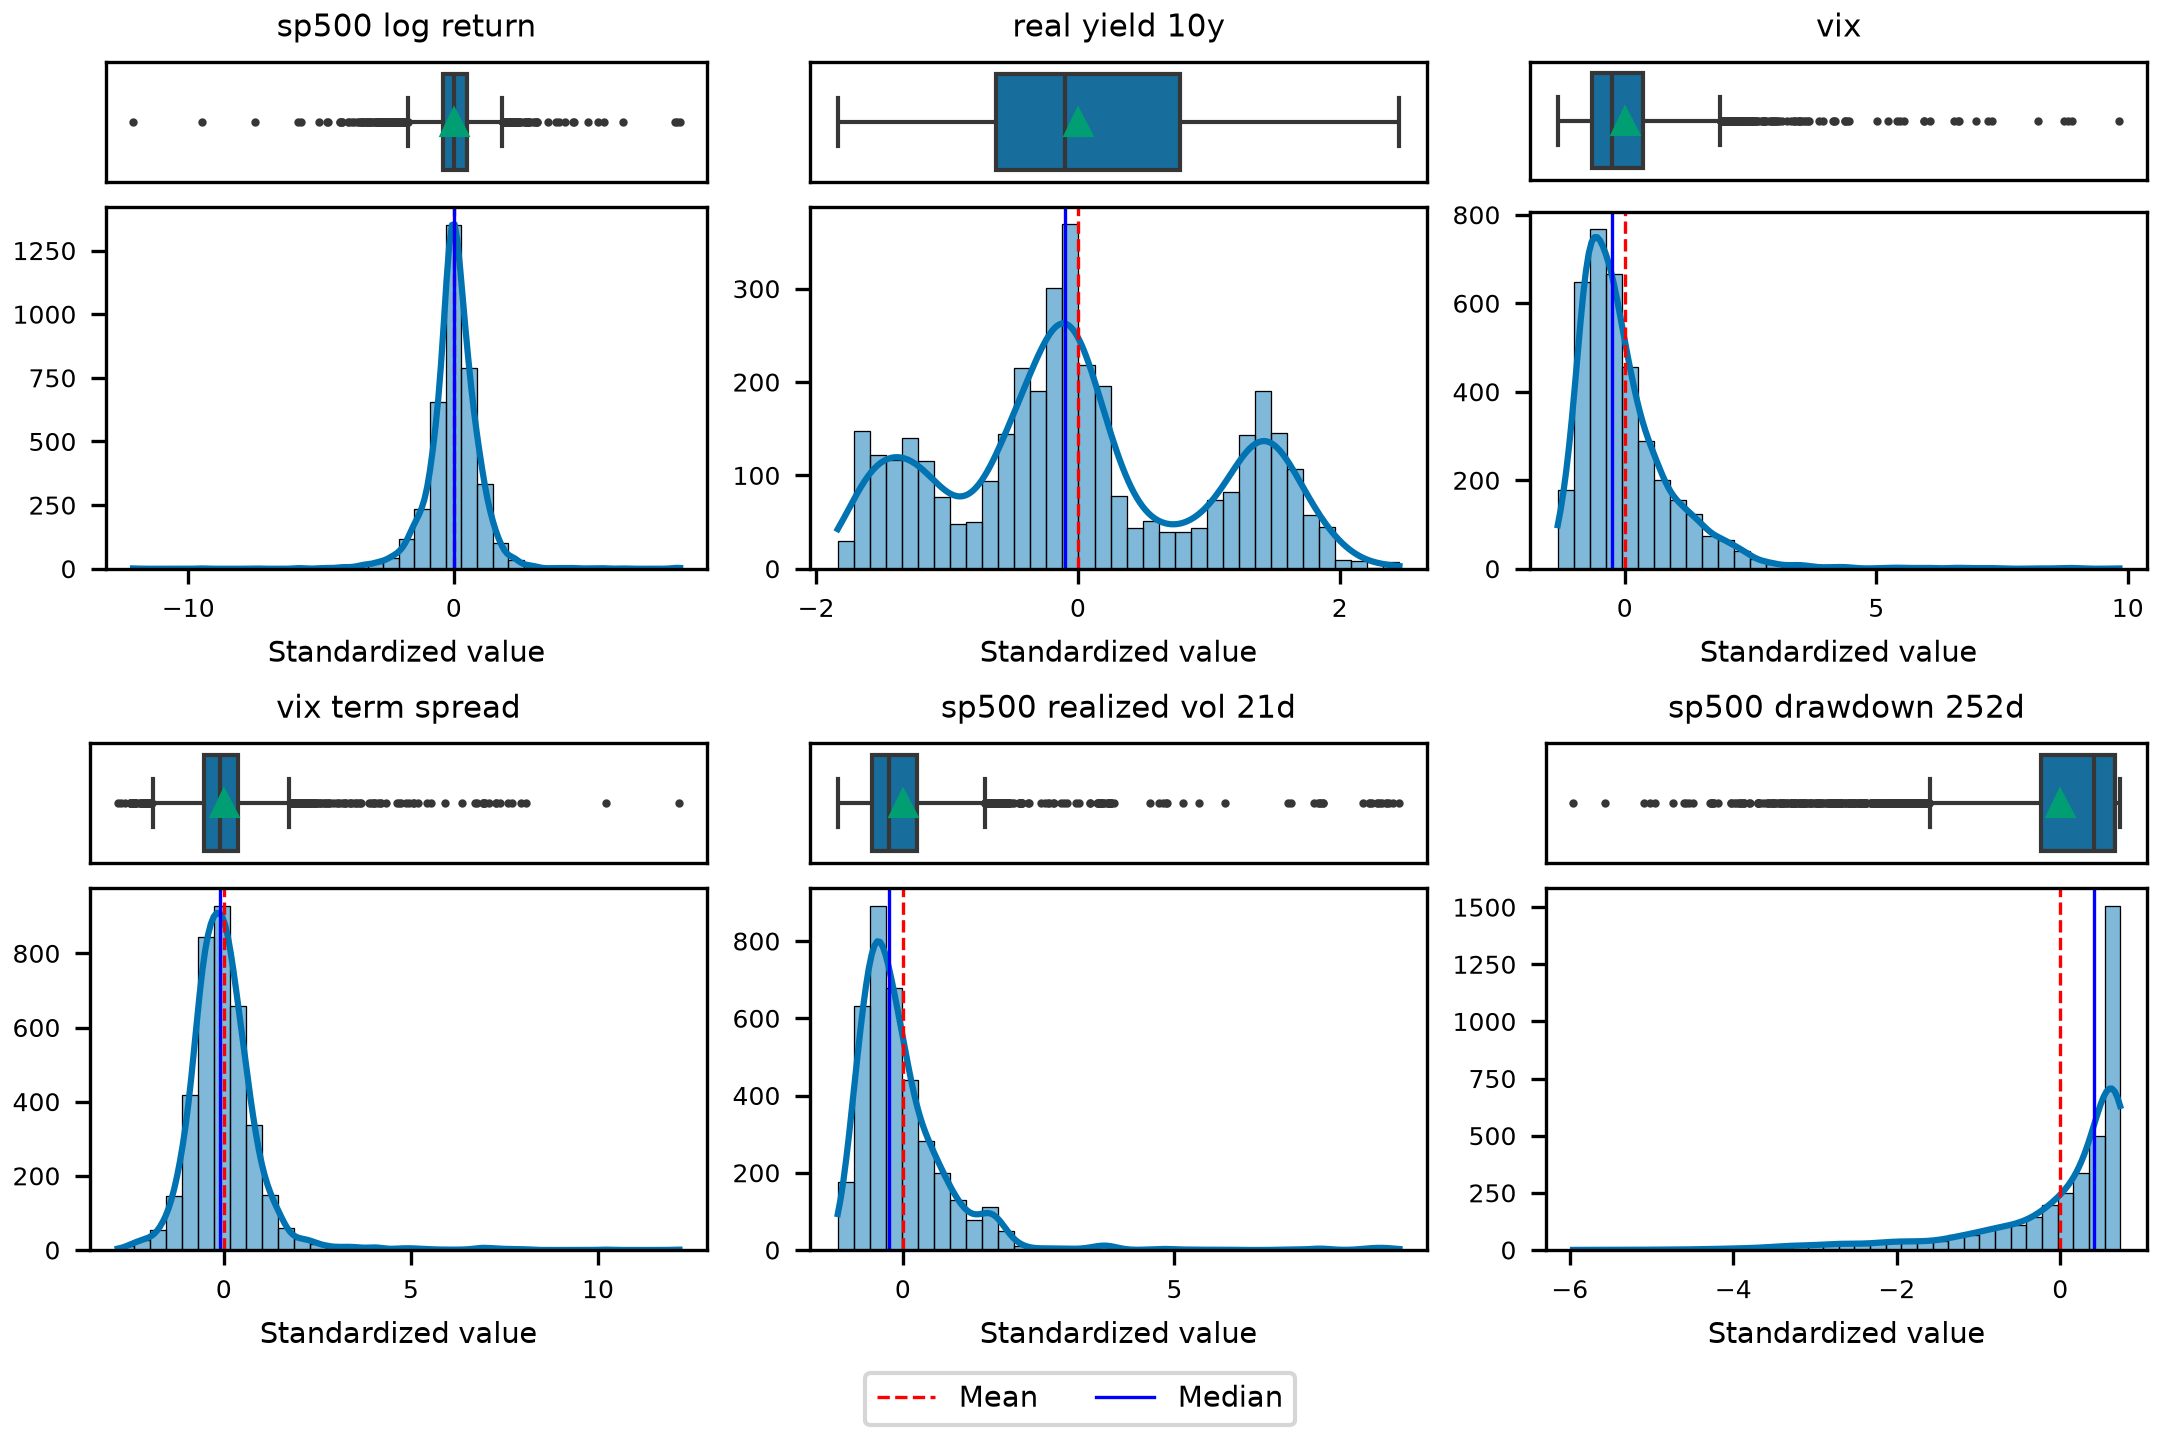
\includegraphics[width=\textwidth]{images/scaled_feature_distributions.png}
\caption{Selected feature distributions after StandardScaler, with a horizontal boxplot above each histogram. All horizontal axes are in standardized units. Red dashed lines mark means and blue lines mark medians. The full 17-feature diagnostic is included in the notebook immediately after scaling.}
\label{fig:scaled-distributions}
\end{figure}

Mixed feature definitions are not inherently inconsistent: the output return is a resampled asset increment, while the conditioning inputs describe market states. Neither the empirical EP formulation nor the K-means objective requires Gaussian marginal distributions. The methodological concern is how skewness, tails and related volatility features influence PCA covariance and squared Euclidean distances. A stress-versus-calm partition may partly reflect those choices.

Alternative feature maps, such as log levels of strictly positive volatility measures or changes in yields where economically appropriate, should be compared as separate configurations with renewed PCA and cluster selection. A log level is not a log return, and no automatic clipping or additional transformation is applied here. Histograms alone do not establish stationarity; state persistence, structural change and out-of-sample stability also require evaluation.

\subsection{PCA covariance and score transformation}

Apply PCA to the scaled, mean-centred vectors $\widetilde y_t$. Write the eigendecomposition of their sample covariance as
\begin{equation}
\widehat\Sigma=\frac{1}{T-1}\sum_{t=1}^{T}\widetilde y_t\widetilde y_t^\top
=V\Lambda V^\top,
\qquad \lambda_1\geq\cdots\geq\lambda_p\geq0.
\end{equation}

Choose $\widehat L$ using equation~\eqref{eq:pca-dimension}. The input received by K-means is then
\begin{equation}
u_t=V_{\widehat L}^{\top}\widetilde y_t\in\mathbb R^{\widehat L},
\label{eq:pca-scores}
\end{equation}
Here $V_{\widehat L}$ contains the eigenvectors associated with the retained eigenvalues. No whitening is applied. These score vectors form the rows of $U_{\widehat L}$ in the main pipeline; candidate K-means models are fitted in this representation.

\section{Complete model and calibration inventory}
\label{app:model-inventory}

Table~\ref{tab:original-inventory} retains all five starting fits, five original standard-input selections and ten fixed-settings PCA95/robust checks from notebook 02. The historical rows are preserved, including small-cluster and unavailable-score outcomes. They are not silently replaced by the retrospective screened selections in Table~\ref{tab:original-selected-models}. In particular, the original hierarchical calibration checks inherit complete linkage; they are not robust/PCA95 checks of the newly reported screened Ward alternative. DBSCAN recalibrates its selected neighbour-distance quantile in each representation.

The source snapshots are stored alongside this document in \texttt{tables/original\_model\_comparison.csv} and \texttt{tables/original\_tuning\_trials.csv}; the screened per-model selections are in \texttt{tables/original\_screened\_selections.csv}. They preserve the original notebook eligibility flag and add a separately named paper-population-screen flag. The CSV files include the full metrics and parameter dictionaries, while the printed inventory emphasizes silhouette, population and coverage. The snapshots do not require the ignored local data directory to compile this paper.

\begin{table}[htbp]
\centering
\footnotesize
\begin{tabularx}{\textwidth}{@{}Xllrrrrc@{}}
\toprule
Model & Stage & Input & $K$ & Sil. & Min. $N_k$ & Cover. & Screen\\
\midrule
K-means & Base & Standard & 3 & 0.174 & 635 & 100.0 & Yes\\
K-means & Tuned & Standard & 2 & 0.329 & 739 & 100.0 & Yes\\
K-means & Check & PCA95 & 2 & 0.329 & 738 & 100.0 & Yes\\
K-means & Check & Robust & 2 & 0.342 & 671 & 100.0 & Yes\\
K-medoids & Base & Standard & 3 & 0.165 & 619 & 100.0 & Yes\\
K-medoids & Tuned & Standard & 8 & 0.171 & 213 & 100.0 & Yes\\
K-medoids & Check & PCA95 & 8 & 0.170 & 246 & 100.0 & Yes\\
K-medoids & Check & Robust & 8 & 0.164 & 198 & 100.0 & Yes\\
Hierarchical & Base & Standard & 3 & 0.142 & 746 & 100.0 & Yes\\
Hierarchical & Tuned & Standard & 2 & 0.739 & 9 & 100.0 & No\\
Hierarchical & Check & PCA95 & 2 & 0.665 & 18 & 100.0 & No\\
Hierarchical & Check & Robust & 2 & 0.711 & 22 & 100.0 & No\\
GMM & Base & Standard & 3 & 0.147 & 790 & 100.0 & Yes\\
GMM & Tuned & Standard & 8 & 0.153 & 39 & 100.0 & Yes\\
GMM & Check & PCA95 & 8 & 0.138 & 63 & 100.0 & Yes\\
GMM & Check & Robust & 8 & 0.145 & 69 & 100.0 & Yes\\
DBSCAN & Base & Standard & 1 & --- & 3687 & 98.6 & No\\
DBSCAN & Tuned & Standard & 4 & 0.103 & 24 & 92.0 & No\\
DBSCAN & Check & PCA95 & 3 & 0.114 & 37 & 91.9 & No\\
DBSCAN & Check & Robust & 5 & 0.097 & 19 & 91.2 & No\\
\bottomrule
\end{tabularx}
\caption{All 20 configurations originally displayed in notebook 02. Coverage is a percentage. ``Screen'' applies the retrospective paper rule, not notebook 02's original eligibility flag. The hierarchical tuned row is the original complete-linkage winner; its PCA95/Robust checks inherit those settings. The screened Ward alternative in Table~\ref{tab:original-selected-models} is recovered from the full saved grid. PCA95 and robust rows keep each original standard winner's settings rather than repeating the search.}
\label{tab:original-inventory}
\end{table}

\clearpage

\section{Robustness and statistical profile comparisons: methodological notes}
\label{app:profile-inference}
\setcounter{equation}{0}

This appendix is a methods outline for the extended study in Section~\ref{sec:evaluation}. It contains no empirical results. Split dates, gaps, eligibility rules, covariance bandwidths and the family of hypotheses should be documented before interpreting the comparisons.

\subsection{Conditional profiles under a learned assignment rule}

For feature draw $b$, let $\widehat g_b$ denote the preprocessing and assignment rule fitted on training observations, with selected count $\widehat K_b$. For an evaluation observation define $C_b=\widehat g_b(y)$ and let $Z_j$ be variable $j$ in the common profile panel. The relevant conditional quantities are
\begin{equation}
\mu_{kj}^{(b)}=\mathbb E[Z_j\mid C_b=k],
\qquad
v_{kj}^{(b)}=\operatorname{Var}(Z_j\mid C_b=k),
\quad k=0,\ldots,\widehat K_b-1.
\end{equation}
The clustering representation and the profiled variable need not use the same units or transformation. In particular, recover an equity simple return as $R=\exp(r)-1$ and define its loss as $L=-R$. Write $a_{\alpha,k}^{(b)}$ for the conditional loss quantile at level $\alpha$. Expected shortfall is
\begin{equation}
\mathrm{ES}_{\alpha,k}^{(b)}
=a_{\alpha,k}^{(b)}+
\frac{\mathbb E[(L-a_{\alpha,k}^{(b)})_+\mid C_b=k]}{1-\alpha},
\label{eq:profile-es}
\end{equation}
where $(x)_+=\max(x,0)$ \cite{rockafellaruryasev2000}. This loss convention makes larger CVaR values represent worse tail losses. Its empirical version accounts for fractional mass at a quantile boundary.

\subsection{Hypotheses and dependence-aware comparison}

For each draw and variable, the proposed hypotheses are
\begin{align}
H_{0,\mu,j}^{(b)} &: \mu_{0j}^{(b)}=\cdots=\mu_{\widehat K_b-1,j}^{(b)},\\
H_{0,v,j}^{(b)} &: v_{0j}^{(b)}=\cdots=v_{\widehat K_b-1,j}^{(b)},\\
H_{0,\mathrm{ES},\alpha}^{(b)} &: \mathrm{ES}_{\alpha,0}^{(b)}=\cdots=
\mathrm{ES}_{\alpha,\widehat K_b-1}^{(b)}.
\end{align}
Thus the number of hypotheses and their contrasts accommodate a selected count rather than a universal pair of clusters. An omnibus rejection for more than two groups establishes at least one difference, not that every pair differs.

Let $\widehat\theta$ collect the cluster-specific estimates for one characteristic, and let $D$ contrast each cluster with a reference group. With a suitable estimated covariance $\widehat V$ of $\widehat\theta$, the Wald statistic is
\begin{equation}
W=(D\widehat\theta)^\top
\bigl(D\widehat V D^\top\bigr)^{-1}
(D\widehat\theta).
\end{equation}
Under the null and the required regularity conditions, compare $W$ with a $\chi^2_{\widehat K_b-1}$ reference distribution. Estimate covariance from influence functions on the full chronological evaluation sequence using a heteroskedasticity and autocorrelation consistent estimator \cite{neweywest1987}. Preserve time positions when a date belongs to another cluster; concatenating a cluster's dates would distort lag structure. Required moments, tail support, covariance rank and bandwidth sensitivity need explicit checks. HAC adjustment does not resolve structural nonstationarity or ensure finite-sample validity.

\subsection{Multiplicity, eligibility and interpretation}

Declare the correction family across variables, characteristics and feature draws, and report Holm-adjusted p-values alongside unadjusted values \cite{holm1979}. Report unsuccessful training fits, absent evaluation groups, insufficient group or tail populations, and singular covariance estimates without changing the selection rule to obtain testable winners. Distinguish a skipped test from a non-rejection, and include effect sizes and uncertainty summaries rather than significance flags alone.

The inferential target is the conditional profile inside a fixed learned assignment region. When the equity return helps determine that region, rejecting equal return characteristics does not independently demonstrate latent economic regimes or future-return predictability. Interpretation should also distinguish variables used in the fit from omitted variables, and recognize their dependence. Formal profile comparisons complement the separate bootstrap and feature-sensitivity exercises; empirical conclusions are deferred until the design and calibration are settled.

\end{document}
